% -----------------------------------------------
% Template for ISMIR Papers
% 2017 version, based on previous ISMIR templates

% Requirements :
% * 6+n page length maximum
% * 4MB maximum file size
% * Copyright note must appear in the bottom left corner of first page
% * Clearer statement about citing own work in anonymized submission
% (see conference website for additional details)
% -----------------------------------------------

\documentclass{article}
\usepackage{ismir,amsmath,amssymb,cite,url}
\usepackage{graphicx}
\usepackage{color}
\usepackage{cleveref}
\usepackage{graphicx}
\usepackage{color}
\graphicspath{{figs/}}
\usepackage{booktabs}
\usepackage[inline]{enumitem}

\setlist[itemize]{noitemsep, topsep=0ex}
\setlist[enumerate]{noitemsep, topsep=0ex}

\def\eg{\emph{e.g.\/}}
\def\ie{\emph{i.e.\/}}
\def\etc{\emph{etc.\/}}
\def\etal{\emph{et al.\/}}


% Title.
% ------
\title{Structured training for large-vocabulary chord recognition}

% Note: Please do NOT use \thanks or a \footnote in any of the author markup

% Single address
% To use with only one author or several with the same address
% ---------------
%\oneauthor
% {Names should be omitted for double-blind reviewing}
% {Affiliations should be omitted for double-blind reviewing}

% Two addresses
% --------------
%\twoauthors
%  {First author} {School \\ Department}
%  {Second author} {Company \\ Address}

%% To make customize author list in Creative Common license, uncomment and customize the next line
%  \def\authorname{First Author, Second Author}


% Three addresses
% --------------
\threeauthors
  {First Author} {Affiliation1 \\ {\tt author1@ismir.edu}}
  {Second Author} {\bf Retain these fake authors in\\\bf submission to preserve the formatting}
  {Third Author} {Affiliation3 \\ {\tt author3@ismir.edu}}

%% To make customize author list in Creative Common license, uncomment and customize the next line
%  \def\authorname{First Author, Second Author, Third Author}

% Four or more addresses
% OR alternative format for large number of co-authors
% ------------
%\multauthor
%{First author$^1$ \hspace{1cm} Second author$^1$ \hspace{1cm} Third author$^2$} { \bfseries{Fourth author$^3$ \hspace{1cm} Fifth author$^2$ \hspace{1cm} Sixth author$^1$}\\
%  $^1$ Department of Computer Science, University , Country\\
%$^2$ International Laboratories, City, Country\\
%$^3$  Company, Address\\
%{\tt\small CorrespondenceAuthor@ismir.edu, PossibleOtherAuthor@ismir.edu}
%}
%\def\authorname{First author, Second author, Third author, Fourth author, Fifth author, Sixth author}


\sloppy % please retain sloppy command for improved formatting

\begin{document}

%
\maketitle
%
\begin{abstract}
Automatic chord recognition systems operating in the large-vocabulary regime must overcome data scarcity: certain classes occur much less frequently than others, and this presents a significant challenge when estimating model parameters.
While most systems model the chord recognition task as a (multi-class) classification problem, few attempts have been made to directly exploit the intrinsic structural similarities between chord classes.

In this work, we develop a deep convolutional-recurrent model for automatic chord recognition over a vocabulary of 170 classes.
To exploit structural relationships between chord classes, the model is trained to produce both the time-varying chord label sequence as well as binary encodings of chord roots and qualities.
This binary encoding directly exposes similarities between related classes, allowing the model to learn a more coherent representation of acoustic harmony.
Evaluations on a corpus of 1217 annotated recordings demonstrate substantial improvements compared to previous models.
\end{abstract}
%
\section{Introduction}\label{sec:introduction}

% Chord recognition is maturing as a problem within MIR

% The gains to be had are now in the large-vocab regime (eg, tetrads/sevenths)

% These classes are rare in the common datasets, so modeling them is hard

% But we can leverage the structure of chord space to better exploit available data

\subsection{Our contributions}

We develop convolutional-recurrent neural networks for large-vocabulary chord recognition.
To exploit similarity between target chord classes, we introduce a structured representation which influences the intermediate representation and informs the output label predictor.
By combining deep, recurrent networks with structured representation learning, the proposed models achieve substantially higher accuracy than previous models based on convolutional networks and hidden Markov models.

%
\section{Related work}

Chord recognition has received a substantial amount of attention in the MIR literature, and a comprehensive survey of existing methods is beyond the scope of this paper.
Here, we highlight the work that are most closely related to the proposed methods in this paper.

%%% structured HMM methods
Hidden Markov models (HMMs) have been a popular method for designing chord recognition systems, and provide a flexible framework in which to integrate musical domain knowledge.
The general HMM approach models chord identities as latent state variables to be inferred from observed time-series features (\eg, chroma vectors).
Systems like Chordino~\cite{mauchsimple} and HPA~\cite{ni2012end} extend this idea by introducing additional latent variables to model key, bass, and metrical position.
In these systems, bass is modeled by weighting or partitioning the frequency range to produce distinct \emph{bass} and \emph{treble chroma} observations.
The $K$-stream HMM takes this idea a step further by modeling $K$ distinct frequency sub-bands, though it does not explicitly infer bass~\cite{cho2014improved}.
The structured representation we describe in \cref{sec:methods} differs in that root, bass, and chord quality are jointly inferred from the entire spectrum, and it makes no assumptions about absolute height.

% 2010 - chordino, 159 but not quite the same
%   bass / treble tracking (pre-determined split)
%   no explicit root model
%   latent key model
%   metrical position + HMM dynamics
%   large vocab
%\cite{mauchsimple}

% 2012 - HPA (bass tracking), 25-class, 121-class
%   HPA did bass tracking
%   key, bass, root modeling
%   explicit partition of bass / treble by frequency
%   HMM for dynamics
%\cite{ni2012end}

% 2014 - TMC (157)
%   independent hmms per sub-band
%   
%\cite{cho2014improved} 

%%% Deep methods
In recent years, deep learning methods have been increasingly popular for chord recognition.
The majority of existing systems are trained in two stages. 
First, a model is built first to encode short patches of audio, \eg as an idealized chroma vector~\cite{boulanger2013audio,korzeniowski2016feature} or likelihood distribution over chord categories~\cite{humphrey2015four,sigtia2015audio,zhou2015chord,deng2016hybrid}.
Second, a dynamics model integrates the time-series of learned representations to produce a sequence of predicted labels, \eg using an HMM~\cite{humphrey2015four,zhou2015chord}, recurrent neural network (RNN)~\cite{boulanger2013audio,sigtia2015audio}, or simple point-wise prediction~\cite{korzeniowski2016feature}.
The models proposed in this work differ in that they are jointly trained end-to-end from spectral features, and learn the internal representation along with the dynamics using multiple recurrent layers.

Regardless of the model architecture, it is common to exploit some structural properties of chords, \eg by tying model parameters for the same chord quality across roots~\cite{humphrey2015four}, or rotating chroma vectors through all possible root positions during training~\cite{cho2014improved}.
Although the methods we propose do not model quality independent of root, they do model active pitch class sets independently.
Chroma rotation can be viewed as a form of data augmentation, and the models we develop benefit substantially from a slightly more general form of augmentation described in \cref{sec:muda}.
To the best of our knowledge, the proposed method is the first to exploit similarities between chords by jointly modeling labels and structured encodings.

% 2016 - idealized chroma prediction
%   cqt patch -> center frame idealized chroma
%   idealized chroma -> logistic regression on small vocab
%   not trained end-to-end
%   small vocab
%\cite{korzeniowski2016feature}

% 2013 
%   stft frame -> idealized chroma
%   idealized chroma -> rnn
%   supposedly large vocab, though no results
%\cite{boulanger2013audio}

% 2015 - four timely lessons (157)
%       cqt patch -> cnn -> center frame chord prediction
%       prediction sequence -> hmm
%       not trained end-to-end
%\cite{humphrey2015four}

% 2015 - sigtia, RNN
%       small vocab
%       cqt patch -> dnn -> center frame chord prediction
%       prediction sequence -> rnn
%       not trained end-to-end
%\cite{sigtia2015audio} 


%%% Deep but unstructured

% 2015 - zhou
%\cite{zhou2015chord}

% 2016 - deng
%   recurrent networks over very short patches
%   predict chord label of center frame
%   large vocab
%\cite{deng2016hybrid}



\section{Methods}
\label{sec:methods}
% Use convolutional filters for local representation

% Use a bidrectional recurrent model to capture dynamics

% Predict chord label from latent state representation

%% either directly

%% or by first estimating (root, pitch classes, bass)

This section outlines the data preparation, architectures, and training strategies for the models under comparison.
We consider three independent design choices: one or two recurrent layers, the presence or absence of data augmentation, and the presence or absence of structured output training.
This results in eight model configurations, which are evaluated in the subsequent section.

\subsection{Encoder-decoder models}

The basic model architecture depicted in \cref{fig:crnn1} follows a convolutional encoder, recurrent decoder architecture.
The \emph{encoder} component maps audio into a latent feature space using only local information, while the \emph{decoder} component maps from the latent feature space to the output space, and uses the entire available observation for context.

Input audio is represented as a $T\times F$ time-series of log-power constant-Q spectra (for $T$ frames and $F$ frequency bands).
After batch normalization~\cite{ioffe2015batch} (not pictured), the first convolutional layer consists of a single two-dimensional $5\times5$ filter, followed by a bank of $36$ single-frame, one-dimensional convolutional filters, resulting in a $T\times 36$ feature encoding.
Both layers use rectified linear (ReLU) activations.
The first layer can be interpreted as a local harmonic saliency enhancer, as it tends to produce a filter which suppresses transients and vibrato while emphasizing sustained tones.
The second layer produces a convolutional encoding of the harmonic content of each frame.

\begin{figure}
    \centering
    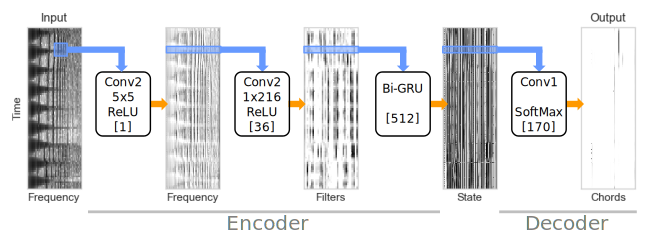
\includegraphics[width=\columnwidth]{crnn1}
    \caption{The convolutional encoder, recurrent decoder network denoted as \emph{CR1}.
            Each CQT frame is filtered by a single $5\times 5$ 2D-convolutional filter, and then encoded as a set of 36 1-D filter activations.
            The bi-directional recurrent decoder integrates across the entire observation to produce a time-series of 512-dimensional hidden state vectors. 
            Each hidden state vector is independently decoded to its most likely chord label.\label{fig:crnn1}}
\end{figure}


The convolutional feature encoding is mapped into either one or two layers of bi-directional gated recurrent units (GRUs)~\cite{cho2014learning}.
The GRU model is functionally similar to the commonly used long-short-term memory (LSTM) model~\cite{hochreiter1997long}, but has fewer parameters and often performs comparably in practice~\cite{jozefowicz2015empirical}.
For a sequence of $d$-dimensional input vectors $x(t) \in \mathbb{R}^d$, the GRU produces a sequence of $D$-dimensional hidden state vectors $h(t) \in [-1, +1]^D$ as follows:
\begin{eqnarray}
    r(t) &=& \sigma\left(W_r x(t) + T_r h(t-1) + b_r\right)\\
    u(t) &=& \sigma\left(W_u x(t) + T_u h(t-1) + b_u\right)\\
    \hat{h}(t) &=& \rho\left(W_h x(t) + T_h \left( r(t) \odot h(t-1) \right) + b_h \right)\label{eq:candidate}\\
    h(t) &=& u(t) \odot h(t-1) + (1-u) \odot \hat{h}(t),
\end{eqnarray}
where $r(t), u(t) \in [0,1]^D$ are the \emph{reset} and \emph{update} vectors, each of which are controlled by RNN dynamics depending on the input $x$ and previous hidden state $h$, and $\rho$ is a non-linear activation (typically $\tanh$).
When an element of the update vector ${u(t)}_j \approx 1$, the corresponding element of the previous hidden state is copied directly to the current state ${h(t)}_j \leftarrow {h(t-1)}_j$.
Otherwise, if $r(t) \approx 1$, then $h(t)$ evolves according to standard RNN dynamics.
However, when $r(t) \approx 0$, the $h$ term in~\eqref{eq:candidate} goes to 0 and the update \emph{resets} and depends only on the input $x(t)$.
In this way, the GRU model can persist a hidden state across arbitrary long spans of time, and encode variable-length temporal dependencies.
These properties make the GRU model appealing for chord recognition, where temporal dependencies are often variable, long-range, and subject to sudden changes rather than gradual evolution.

The bi-directional variant consists of two independent GRUs, one running in each direction, whose hidden state vectors are concatenated to produce the bi-directional hidden state vector $h(t)$.
This layer integrates over the entirety of the input signal, and provides temporal smoothing and context for the encoded feature representation.

% TODO:
%   explain the 1-vs-2 decision
%       local smoothing vs long-range interactions
%       breadth vs depth

In the one-layer configuration (denoted as \emph{CR1}), the hidden state vector has total dimension 512 (256 for each direction).
In the two-layer configuration (denoted as \emph{CR2}), both layers have total hidden state dimensions 256, and the hidden state of the first layer serves as input to the second layer.


The final hidden state vector $h(t)$ is decoded to the class label by a sigmoid layer, which produces a likelihood score $\hat{y}(t) \in [0, 1]^{V}$ over the chord vocabulary of $V$ symbols.
At each frame, the maximum likelihood label is selected, and the time-series of chord labels is run-length encoded to form the estimated annotation for the track.


% Figure for the basic model

% conv encoder, recurrent decoder model

% batch-norm on the cqt for standardization

% first filter = transient suppressor / local salience

% 3*12 full-height convolutional filters

% bidirectional recurrent model (GRU), d=128 in each direction

% logistic to output vocabulary


\subsection{Chord vocabulary}

\label{sec:vocab}
% For training the tag decoder, we map to a fixed vocabulary
%   1. discard missing / extra notes
%   2. discard inversions
%   3. split into (root, pitch classes)
%   4. match against quality templates:
%       - N
%       - maj, min, dim, aug
%       - min6, maj6
%       - min7, maj7, dom7, dim7, hdim7, minmaj7
%       - sus2, sus4
%       - X (unmatched)
%   5. resulting vocab = 12 * 14 + 2 = 170 classes
%

To formulate chord recognition as a classification task, we define a mapping of all valid chord descriptions to a finite vocabulary by the following procedure.\footnote{Here, a \emph{valid chord} is any string belonging to the formal language specification of Harte~\emph{et al.}~\cite{harte2005symbolic}, or the extended grammar implemented in the JAMS library~\cite{humphrey2014jams}.}
First, suppressed or extra notes are discarded, \eg:
\begin{align*}
    \texttt{D}\flat\texttt{:maj(*5,9)/3} &\mapsto \texttt{D}\flat\texttt{:maj/3}.
\end{align*}
Inversions are then discarded, \eg:
\begin{align*}
    \texttt{D}\flat\texttt{:maj/3} &\mapsto \texttt{D}\flat\texttt{:maj}.
\end{align*}
Next, labels are decomposed into \emph{root} and \emph{pitch classes} (relative to the root) using the encoding functionality provided by \texttt{mir\_eval}~\cite{raffel2014mir_eval}, \eg:
\begin{align*}
    \texttt{D}\flat\texttt{:maj} &\mapsto \begin{cases}
        1 & \text{root}\\
        (0, 4, 7) & \text{pitch classes}
    \end{cases}.
\end{align*}
The set of active pitch classes is matched against a set of 13 templates: \texttt{maj, min, dim, aug, min6, maj6, min7, maj7, dom7, hdim7, minmaj7, sus2, sus4}.
The root and matched template are combined, and mapped to a canonical form to resolve enharmonic equivalences:
\begin{align*}
    \left(1, (0, 4, 7) \right) &\mapsto \texttt{C}\sharp\texttt{:maj}.
\end{align*}
If the pitch class set does not match one of the templates, it is mapped to the unknown chord symbol \texttt{X}; the no-chord symbol is represented distinctly as \texttt{N}.
The final vocabulary contains 170 classes: 2 special symbols (\texttt{N, X}), and $12\times13=168$ combinations of root and quality.


\subsection{Structured training}

% Figure for the structured model

% Note: for structured training, no simplification is performed
%       so that the model can still learn to map power chords to major, for example
%       but the decoder component is still trained to map to the constrained vocab
%       even for chords that are out of vocab, we can still learn from their encoded representation 
%       and map them onto to a plausible output
%       

The CR models described above map each hidden state vector to a fixed vocabulary produced by the chord simplification strategy described in \cref{sec:vocab}.
They can be optimized in the usual way by minimizing a multi-class classification loss (cross-entropy), but this approach has two clear drawbacks.
First, it does not leverage the structure of chord space: for example, if the model predicts \texttt{B:maj} instead of \texttt{B:7}, it is penalized just as much as if it had predicted \texttt{C:maj} or \texttt{N}, even though it is far less severe of a mistake.
Second, the chord simplification strategy is \emph{lossy} in that it discards information such as suppressed or additional notes, which can render certain chords ambiguous, such as power chords like \texttt{A:maj(*3)}$\mapsto$\texttt{A:maj}.
These effects combine to inhibit the model's ability to capture certain classes.

To counteract these effects, we introduce a structured representation to the decoder component of the model, depicted in \cref{fig:crnn2}.
The standard evaluation criteria for chord recognition operate over a decomposed representation of (\emph{root}, \emph{pitch classes}, \emph{bass}), as described in \cref{sec:vocab}~\cite{raffel2014mir_eval}.
This representation can be predicted directly by the model, and used either as direct output, or as an intermediate representation prior to predicting the chord label.

% TODO:
%   in this space, common disagreements eg C:maj vs C:7 have some structural similarity due to common root and pitches
%   this is explicitly integrated in our model

The structured models (denoted as \emph{CR1/2+S}) predict for each frame $t$ the root pitch class (\texttt{C}--\texttt{B}, plus \texttt{N} for no-root), the bass pitch class, and the active pitch classes from the hidden state vector $h(t)$.
Root and bass estimation are modeled as a multi-class prediction with a soft-max non-linearity.
Pitch class prediction is modeled as a multi-label prediction, and uses a logistic (sigmoid) non-linearity.
This results in an idealized chroma representation similar to that of Korzeniowski and Widmer~\cite{korzeniowski2016feature}, but predicted from the hidden state of an RNN rather than a spectrogram patch.
These three layers are concatenated, along with the hidden state itself, to produce the structured representation from which the chord label is predicted.

\begin{figure}
    \centering
    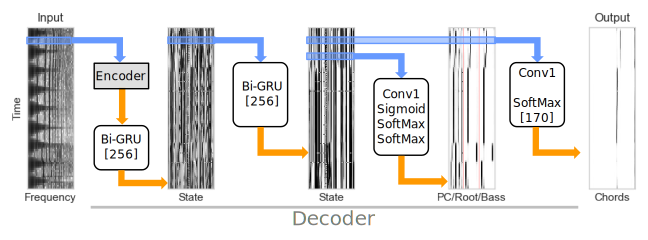
\includegraphics[width=\columnwidth]{crnn2}
    \caption{The structured convolutional encoder, recurrent decoder network, denoted as \emph{CR2+S}.
    The encoder uses the same architecture depicted in \cref{fig:crnn2}.
    The deep decoder (\emph{CR2}) uses two bi-directional recurrent decoders to integrate information across time.
    The structured model (\emph{CR2+S}) predicts the active pitch classes, root, and bass from the second recurrent layer's hidden state.
    The hidden state, root, pitch classes, and bass predictions are then concatenated and used as inputs to the chord prediction layer.\label{fig:crnn2}}
\end{figure}


During training, the structured models are provided with both the simplified chord tag, and the structured representation of the original (non-simplified) chord, and minimize the sum of losses across all outputs.
In this way, the model can both leverage the structure of the output space, and learn to be robust to errors or ambiguities in the vocabulary simplification process.



\subsection{Data augmentation}
\label{sec:muda}
% MUDA
%   training set is augmented with pitch shifts of +- n semitones for n in {1,2,\dots, 6}
%   muda does annotation deformation as well
% all augmentations of a track get the same importance weight
To increase training set variability, we apply pitch-shifting data augmentation using MUDA~\cite{mcfee2015software}.
For each training example, 12 deformations are generated by shifting up or down by between 1--6 semitones.
Testing and validation examples are not augmented.
Because each observation exists in all twelve root classes, this provides a brute-force, approximate root invariance to the model.
Models trained with data augmentation are denoted by \emph{+A}.


\section{Evaluation}

% cite: ejh2015
%   1217, using the same 5-fold CV splits for comparison purposes
%   each training fold is split 75/25 for validation
%   training set => 12x by data augmentation
For evaluation, we used the dataset described by Humphrey and Bello~\cite{humphrey2015four}, which includes 1217 tracks from the Isophonics, Billboard, RWC Pop, and MARL collections.
To facilitate comparison with previous work, we retain the same 5-fold cross-validation splits, and randomly hold out 1/4 of each training set for validation.

\subsection{Pre-processing}

% features
%   librosa 0.5
Feature extraction was performed with librosa 0.5.0~\cite{librosa050}.
%   log cqt power, 36bpo, (C1 - C7) (260 bins)
Each track was represented as a log-power constant-Q spectrogram with 36 bins per octave, spanning 6 octaves starting at C1, and clipped at 80dB below the peak power for the entire track.
%   sr=44100, hop = 4096 => ~96ms frame rate
Signals were analyzed at 44.1KHz with a hop length of 4096 samples, resulting in a frame rate of approximately 10.8Hz.

\subsection{Training}
% training setup
All models are trained on 8-second patches (86 frames), though the models directly generalize to arbitrarily long inputs.
For tracks with multiple reference annotations, the output is selected uniformly at random from all references for each patch.
%   8sec patches (83 frames)
%   32 patches per batch
%   512 batches per epoch
Models are trained using mini-batches of 32 patches per batch, and 512 batches per epoch.
%   ADAM optimization
We use the ADAM optimizer~\cite{kingma2014adam}, and reduce the learning rate if there is no improvement in validation score after 10 epochs.
Training is stopped early if there is no improvement in validation score after 20 epochs, and limited to a maximum of 100 epochs total.
For all models, validation score is determined only by decoder loss (cross-entropy).

%   validation by decoder loss
%   learning rate reduction after 10 epochs
%   early stopping after 20 epochs
%   maximum 100 epochs

%   Keras + tensorflow
All models were implemented with Keras~2.0 and Tensorflow~1.0~\cite{chollet2015keras, tensorflow2015-whitepaper}.\footnote{Source code and pre-trained model parameters for our experiments will be made available upon publication.}

\subsection{Results}

The main results of the evaluation are listed in \cref{fig:results}, which illustrates the median weighted recall scores achieved by each model.\footnote{The trends for the mean scores are qualitatively similar, but the scores are lower for all models. We report the median here to reduce the influence of erroneous or otherwise spurious reference annotations reported by Humphrey and Bello~\cite{humphrey2015four}.}
\begin{figure*}[t]
    \centering
    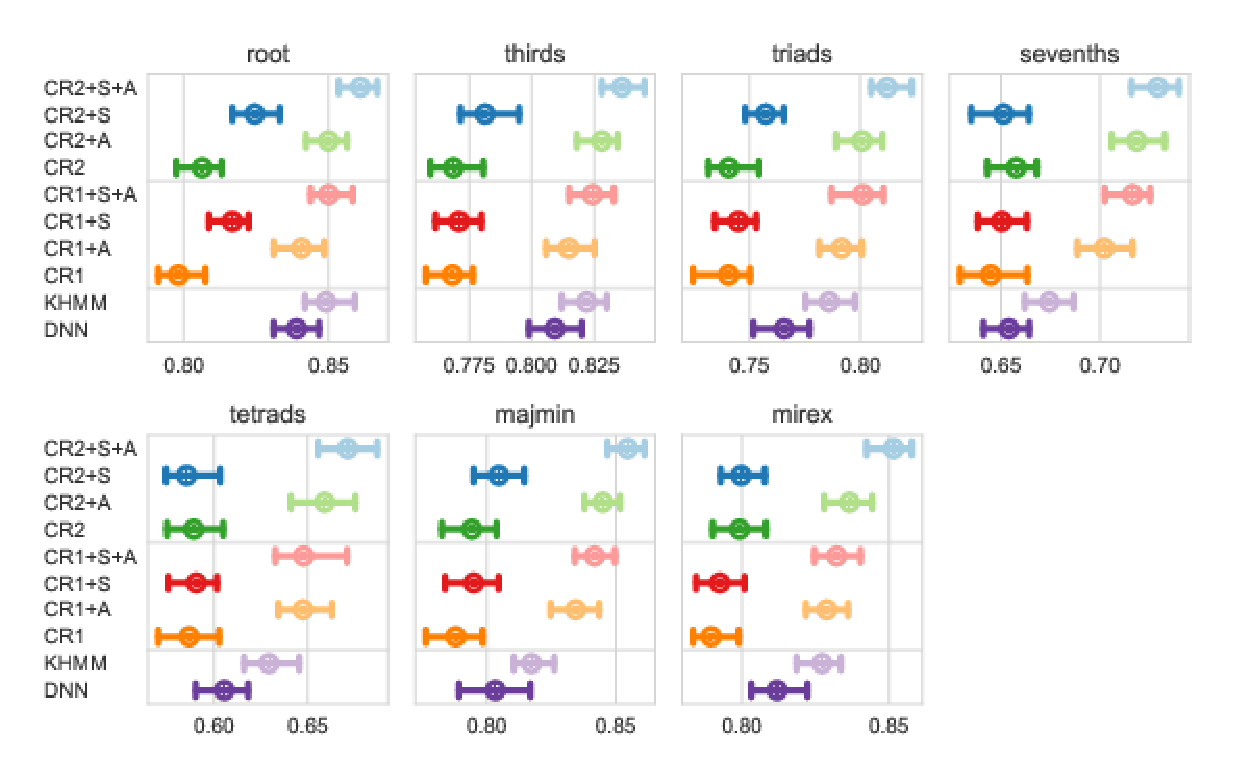
\includegraphics[width=0.9\textwidth]{crnn-scores}
    \caption{Weighted recall scores for all methods under comparison.  Each point represents the median score across all test points, with error bars covering the 95\% confidence interval estimated by bootstrap sampling.
        \emph{KHMM} denotes the K-stream HMM of Cho~\cite{cho2014improved}; \emph{DNN} denotes the convolutional network of Humphrey and Bello~\cite{humphrey2015four}.\label{fig:results}}
\end{figure*}
Each subplot reports the recall computed by \texttt{mir\_eval} of correctly estimating the following:
\begin{itemize}
    \item \emph{root};
    \item \emph{thirds}: root and third;
    \item \emph{triads}: root, third, and fifth;
    \item \emph{sevenths}: root, third, fifth, and seventh;
    \item \emph{tetrads}: all intervals;
    \item \emph{maj-min}: 12 major, 12 minor, and \texttt{N} class; and
    \item \emph{MIREX}: at least three correct notes.
\end{itemize}

From \cref{fig:results}, several trends can be observed.
First, all models are improved substantially across all metrics by data augmentation.  This is to be expected, since the CR models do not model quality independently of root.
Second, structured training generally provides a modest improvement, and it seems particularly helpful for root estimation.
This also should be expected, as structured training specifically forces the model to estimate the root independently of quality.

% FIXME: verify this after all the numbers are in
Interestingly, the deep decoder model (CR2) only improves over the shallow decoder (CR1) when using structured training.
% XXX: Speculation
%   I think this is because without structured training, rare chords look like noise compared to common chords
%   this can throw off the sequencing
%   OTOH, if you have a structured representation, rare chords (eg, dim7) can be related to related chords (eg, dim)
%   TODO: --> find examples of this happening
%   we'd expect this to hurt most in rare classes, so this generally makes sense given the results
%       what's going on with the boost in maj-min though?
%   TODO: --> figure out which classes we mess up the most
%           --> build a 170x170 confusion matrix

Finally, all variants trained with augmentation perform at least as well as the baseline K-HMM, and substantially better on the harder categories as indicated in the plots for \emph{tetrads} and \emph{sevenths}.
\section{Discussion}

% TODO:
%   feature visualization, analysis
%   error analysis: which tracks does CR2SA perform poorly on?
%       worse than KHMM?
%           '--> Ike & Tina Turner - I wanna take you higher
%   future work

%\section*{Acknowledgments}

% For bibtex users:
\bibliography{refs}

\end{document}
